\documentclass{article}
\usepackage[utf8]{inputenc}
\usepackage{amsmath}
\usepackage{amsfonts}
\usepackage{geometry}
\geometry{a4paper, margin=1in}
\usepackage{listings}
\usepackage{xcolor}
\usepackage{tikz}
\usepackage{pgfplots}
\pgfplotsset{compat=1.18} % Recomendado para asegurar la compatibilidad de la gráfica

\title{Modelado Predictivo en la Agroindustria: Regresión y Métricas}
\author{Enfoque: Rendimiento y Calidad de Cultivos}
\date{2026}

\begin{document}

\maketitle

\section{Regresión Lineal Simple: El Cimiento Matemático}

Antes de abordar un ecosistema complejo con múltiples factores, debemos entender el caso bivariado. Supongamos que queremos predecir el rendimiento del cultivo ($y$, en toneladas por hectárea) basándonos en una única variable clave, como la dosis de fertilizante nitrogenado ($x$, en kg por hectárea).

El modelo teórico asume una relación lineal simple:
\begin{equation}
y_i = \beta_0 + \beta_1 x_i + \epsilon_i
\end{equation}

El objetivo del método de \textbf{Mínimos Cuadrados Ordinarios (OLS)} es encontrar los estimadores óptimos $\hat{\beta}_0$ y $\hat{\beta}_1$ que minimicen la suma de los errores al cuadrado. Definimos la Suma de Cuadrados de los Residuos (SCR) como la función a minimizar:
\begin{equation}
SCR(\beta_0, \beta_1) = \sum_{i=1}^{n} \epsilon_i^2 = \sum_{i=1}^{n} (y_i - \beta_0 - \beta_1 x_i)^2
\end{equation}

Para hallar el punto mínimo de esta función (el ``valle'' del error), derivamos parcialmente la función $SCR$ con respecto a $\beta_0$ y $\beta_1$, e igualamos a cero:
\begin{align}
\frac{\partial SCR}{\partial \beta_0} &= -2 \sum_{i=1}^{n} (y_i - \beta_0 - \beta_1 x_i) = 0 \\
\frac{\partial SCR}{\partial \beta_1} &= -2 \sum_{i=1}^{n} x_i(y_i - \beta_0 - \beta_1 x_i) = 0
\end{align}

Al resolver este sistema (conocido como ecuaciones normales), obtenemos las fórmulas algebraicas para nuestros estimadores:
\begin{equation}
\hat{\beta}_1 = \frac{\sum_{i=1}^{n} (x_i - \bar{x})(y_i - \bar{y})}{\sum_{i=1}^{n} (x_i - \bar{x})^2} = \frac{Cov(x,y)}{Var(x)}
\end{equation}

\begin{equation}
\hat{\beta}_0 = \bar{y} - \hat{\beta}_1 \bar{x}
\end{equation}

\section{Ejemplificación Práctica: Datos y Ajuste Visual}

Para ilustrar cómo funciona el método de Mínimos Cuadrados Ordinarios (OLS), imaginemos un pequeño lote experimental donde hemos aplicado diferentes dosis de nitrógeno y medido el rendimiento resultante de la caña.

Tenemos el siguiente conjunto de datos con 5 observaciones:

\begin{table}[h]
\centering
\begin{tabular}{|c|c|c|}
\hline
\textbf{Parcela} & \textbf{Nitrógeno ($x$) [kg/ha]} & \textbf{Rendimiento ($y$) [ton/ha]} \\
\hline
1 & 50 & 45 \\
2 & 70 & 55 \\
3 & 90 & 60 \\
4 & 110 & 75 \\
5 & 130 & 80 \\
\hline
\end{tabular}
\caption{Datos experimentales de rendimiento vs. dosis de nitrógeno.}
\label{tab:datos_ejemplo}
\end{table}

El objetivo de la regresión lineal es trazar una línea recta a través de estos puntos. Sin embargo, como se puede observar en la Figura \ref{fig:ajuste_rectas}, podemos trazar infinitas líneas. ¿Cómo decide el modelo cuál es la ``correcta''?

El método OLS calcula la distancia vertical desde cada punto real hasta la línea propuesta (este es el \textbf{residuo} o error $\epsilon_i$). Luego, eleva cada uno de estos errores al cuadrado y los suma. La recta que produzca la suma total más pequeña (el mínimo cuadrado) es la ganadora.

\begin{figure}[h]
\centering
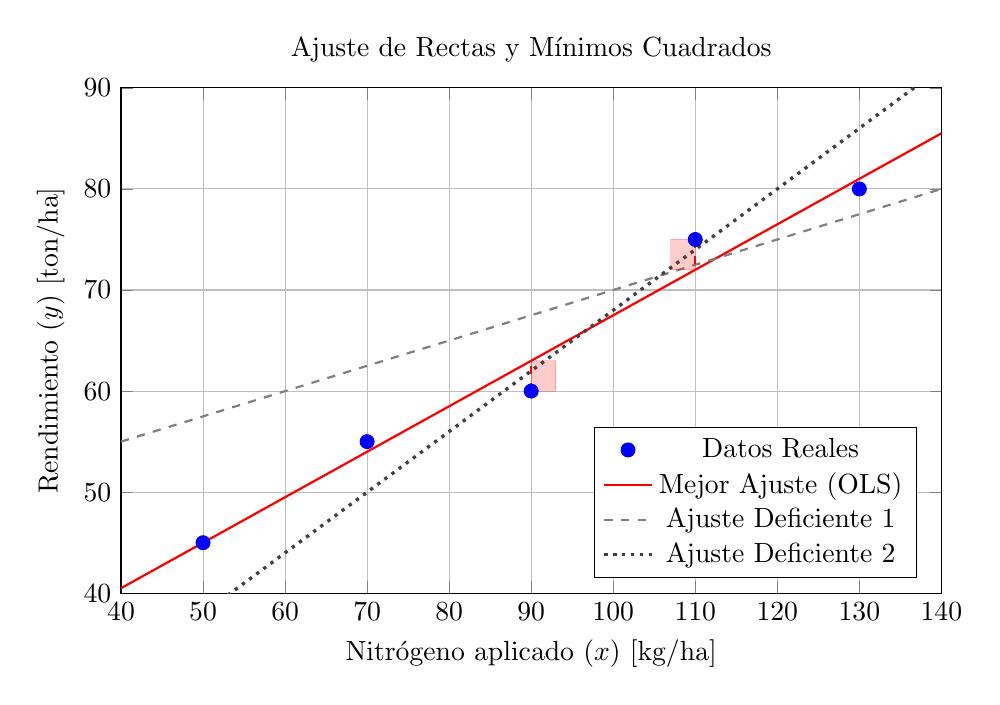
\begin{tikzpicture}
\begin{axis}[
    width=12cm, height=8cm,
    title={Ajuste de Rectas y Mínimos Cuadrados},
    xlabel={Nitrógeno aplicado ($x$) [kg/ha]},
    ylabel={Rendimiento ($y$) [ton/ha]},
    xmin=40, xmax=140,
    ymin=40, ymax=90,
    legend pos=south east,
    grid=major
]

% Puntos de datos reales
\addplot[only marks, mark=*, blue, mark size=2.5pt] coordinates {
    (50,45) (70,55) (90,60) (110,75) (130,80)
};
\addlegendentry{Datos Reales}

% Recta de Mejor Ajuste (OLS): y = 0.45x + 22.5
\addplot[domain=40:140, thick, red] {0.45*x + 22.5};
\addlegendentry{Mejor Ajuste (OLS)}

% Recta deficiente 1 (Subestima la pendiente)
\addplot[domain=40:140, dashed, gray, thick] {0.25*x + 45};
\addlegendentry{Ajuste Deficiente 1}

% Recta deficiente 2 (Sobreestima la pendiente)
\addplot[domain=40:140, dotted, darkgray, very thick] {0.60*x + 8};
\addlegendentry{Ajuste Deficiente 2}

% Representación de los residuos (distancias verticales)
% Para la parcela 3 (90, 60), la recta estima 0.45(90)+22.5 = 63
\draw[red, dashed, thick] (axis cs:90,60) -- (axis cs:90,63);
% Representación visual del "cuadrado" del error
\draw[red, fill=red, opacity=0.2] (axis cs:90,60) rectangle (axis cs:93,63); 

% Para la parcela 4 (110, 75), la recta estima 0.45(110)+22.5 = 72
\draw[red, dashed, thick] (axis cs:110,75) -- (axis cs:110,72);
\draw[red, fill=red, opacity=0.2] (axis cs:110,75) rectangle (axis cs:107,72); 

\end{axis}
\end{tikzpicture}
\caption{Comparación de diferentes rectas de ajuste. La recta roja (OLS) es aquella que minimiza el área total de los cuadrados formados por los residuos (áreas sombreadas).}
\label{fig:ajuste_rectas}
\end{figure}

Al elevar los errores al cuadrado logramos dos cosas cruciales:
\begin{itemize}
    \item Penalizamos de manera desproporcionada los errores muy grandes (un error de 4 pesa 16, no 4).
    \item Evitamos que los errores positivos (puntos por encima de la recta) se cancelen con los negativos (puntos por debajo de la recta).
\end{itemize}

\subsection{Cálculo Manual de los Coeficientes de la Recta}

Para encontrar la recta de mejor ajuste ($y = \hat{\beta}_0 + \hat{\beta}_1 x$), utilizaremos las fórmulas de Mínimos Cuadrados Ordinarios (OLS) derivadas anteriormente, aplicadas a nuestros 5 lotes de caña.

Primero, calculamos las medias muestrales del nitrógeno ($\bar{x}$) y del rendimiento ($\bar{y}$):
$$ \bar{x} = \frac{50 + 70 + 90 + 110 + 130}{5} = \frac{450}{5} = 90 \text{ kg/ha} $$
$$ \bar{y} = \frac{45 + 55 + 60 + 75 + 80}{5} = \frac{315}{5} = 63 \text{ ton/ha} $$

A continuación, necesitamos calcular la covarianza entre $x$ e $y$ (el numerador) y la varianza de $x$ (el denominador). Construimos las sumatorias correspondientes:

\begin{align*}
\sum_{i=1}^{5} (x_i - \bar{x})(y_i - \bar{y}) &= (-40)(-18) + (-20)(-8) + (0)(-3) + (20)(12) + (40)(17) \\
&= 720 + 160 + 0 + 240 + 680 = 1800
\end{align*}

\begin{align*}
\sum_{i=1}^{5} (x_i - \bar{x})^2 &= (-40)^2 + (-20)^2 + (0)^2 + (20)^2 + (40)^2 \\
&= 1600 + 400 + 0 + 400 + 1600 = 4000
\end{align*}

Ahora, calculamos la pendiente ($\hat{\beta}_1$), que representa la tasa de incremento del rendimiento:
$$ \hat{\beta}_1 = \frac{1800}{4000} = 0.45 $$

Finalmente, hallamos el intercepto ($\hat{\beta}_0$), que representa el rendimiento teórico si no se aplicara nitrógeno:
$$ \hat{\beta}_0 = \bar{y} - \hat{\beta}_1 \bar{x} = 63 - (0.45 \times 90) = 63 - 40.5 = 22.5 $$

La ecuación final de nuestra recta de mejor ajuste es:
$$ \hat{y} = 22.5 + 0.45x $$

\textbf{Conclusión del cálculo:} Por cada kilogramo adicional de nitrógeno por hectárea, el modelo estima que el rendimiento de la caña aumentará en 0.45 toneladas, partiendo de una base natural de 22.5 ton/ha.


\textbf{Interpretación Agronómica y Matemática:} 
La ecuación de $\hat{\beta}_1$ nos demuestra que la pendiente de nuestra predicción ($0.45$) depende directamente de cómo covaría el nitrógeno con el rendimiento, normalizado por la varianza del nitrógeno aplicado. Una vez que entendemos esta tasa de cambio, calcular el rendimiento base o intercepto ($\hat{\beta}_0 = 22.5$) es tan sencillo como tomar el rendimiento promedio del lote ($\bar{y} = 63$) y restarle el efecto promedio que tuvo el nitrógeno en ese lote ($\hat{\beta}_1 \bar{x} = 40.5$). En términos agronómicos, la regresión nos permite aislar matemáticamente la capacidad productiva base de la tierra de lo que aporta el fertilizante.
\subsection{Regresión Lineal Múltiple: De la Ecuación a la Matriz}

En un entorno agrícola real, el rendimiento de una parcela $i$ ($y_i$) es el resultado de la interacción simultánea de $k$ factores diferentes (por ejemplo, $x_{1}$ = nitrógeno, $x_{2}$ = precipitación, $x_{3}$ = horas de sol). 

Matemáticamente, ampliamos nuestra ecuación lineal simple para incluir todas estas variables independientes:

$$ y_i = \beta_0 + \beta_1 x_{i1} + \beta_2 x_{i2} + \dots + \beta_k x_{ik} + \epsilon_i $$

Donde:
\begin{itemize}
    \item $y_i$ es el rendimiento observado en la parcela $i$.
    \item $\beta_0$ sigue siendo el intercepto o rendimiento base.
    \item $\beta_j$ (para $j = 1, 2, \dots, k$) son los coeficientes parciales de regresión. Nos indican el cambio en $y_i$ por cada unidad de cambio en $x_{ij}$, asumiendo que el resto de las variables se mantienen constantes (\textit{ceteris paribus}).
    \item $x_{ij}$ es el valor del factor $j$ medido en la parcela $i$.
    \item $\epsilon_i$ es el término de error o perturbación aleatoria.
\end{itemize}

Cuando manejamos cientos de parcelas ($n$ observaciones) y múltiples variables ($k$ predictores), escribir esta ecuación una por una es impráctico. Por ello, la regresión lineal múltiple se expresa de manera mucho más limpia y eficiente utilizando álgebra lineal y notación matricial:

$$ Y = X\beta + \epsilon $$

Desglosando cada componente, tenemos:

$$
\begin{bmatrix}
y_1 \\
y_2 \\
\vdots \\
y_n
\end{bmatrix}
=
\begin{bmatrix}
1 & x_{11} & x_{12} & \dots & x_{1k} \\
1 & x_{21} & x_{22} & \dots & x_{2k} \\
\vdots & \vdots & \vdots & \ddots & \vdots \\
1 & x_{n1} & x_{n2} & \dots & x_{nk}
\end{bmatrix}
\begin{bmatrix}
\beta_0 \\
\beta_1 \\
\vdots \\
\beta_k
\end{bmatrix}
+
\begin{bmatrix}
\epsilon_1 \\
\epsilon_2 \\
\vdots \\
\epsilon_n
\end{bmatrix}
$$

\textbf{Interpretación de las Matrices:}
\begin{itemize}
    \item \textbf{Vector $Y$ ($n \times 1$):} Contiene todas nuestras mediciones históricas de rendimiento.
    \item \textbf{Matriz de Diseño $X$ ($n \times (k+1)$):} Contiene todos nuestros datos de entrada. Nota que la primera columna está compuesta únicamente por unos ($1$); esto es un ``truco'' matemático necesario para poder multiplicar la matriz por el vector $\beta$ y asegurar que el intercepto ($\beta_0$) se sume a cada ecuación.
    \item \textbf{Vector de Parámetros $\beta$ ($(k+1) \times 1$):} Son las incógnitas que nuestro modelo predictivo debe aprender y estimar.
    \item \textbf{Vector de Errores $\epsilon$ ($n \times 1$):} Lo que el modelo no logra explicar.
\end{itemize}
\subsection{El Método de Mínimos Cuadrados en Forma Matricial}

Para encontrar los estimadores óptimos (el vector $\hat{\beta}$), partimos de nuestro vector de errores o residuos, que es la diferencia entre los rendimientos reales observados ($Y$) y los rendimientos que predice nuestro modelo ($X\beta$):

$$ \epsilon = Y - X\beta $$

Queremos minimizar la Suma de Cuadrados de los Residuos ($SCR$). En notación matricial, la suma de los cuadrados de un vector se obtiene multiplicando el vector transpuesto por sí mismo ($\epsilon^T \epsilon$):

$$ SCR(\beta) = \epsilon^T \epsilon = (Y - X\beta)^T (Y - X\beta) $$

Aplicamos las propiedades de transposición de matrices ($(AB)^T = B^T A^T$) para expandir la ecuación:

$$ SCR(\beta) = Y^T Y - Y^T X\beta - (X\beta)^T Y + (X\beta)^T (X\beta) $$
$$ SCR(\beta) = Y^T Y - Y^T X\beta - \beta^T X^T Y + \beta^T X^T X\beta $$

Dado que $Y^T X\beta$ es un escalar (un número único de tamaño $1 \times 1$), su transpuesto es igual a sí mismo, por lo que $Y^T X\beta = \beta^T X^T Y$. Esto nos permite simplificar la ecuación a:

$$ SCR(\beta) = Y^T Y - 2\beta^T X^T Y + \beta^T X^T X\beta $$

Para encontrar el punto mínimo de esta función (el "valle" donde el error es el menor posible), calculamos el gradiente (la derivada vectorial) de $SCR$ con respecto al vector $\beta$ y lo igualamos a cero:

$$ \frac{\partial SCR}{\partial \beta} = -2X^T Y + 2X^T X\beta = 0 $$

Dividimos entre 2 y reorganizamos los términos para obtener las \textbf{Ecuaciones Normales} en su forma matricial:

$$ X^T X\beta = X^T Y $$

Finalmente, para despejar nuestro vector de coeficientes $\hat{\beta}$, multiplicamos ambos lados por la matriz inversa de $(X^T X)$:

$$ \hat{\beta} = (X^T X)^{-1} X^T Y $$

\subsection{Ejemplo Práctico: Resolviendo el Sistema Matricial}

Para aterrizar la ecuación $\hat{\beta} = (X^T X)^{-1} X^T Y$, imaginemos un escenario simplificado, digamos una pequeña evaluación en una finca. Registramos datos de 4 parcelas midiendo el nitrógeno aplicado ($x_1$, en kg/ha), el riego suplementario ($x_2$, en mm) y el rendimiento final ($y$, en ton/ha).

\begin{table}[h]
\centering
\begin{tabular}{|c|c|c|c|}
\hline
\textbf{Parcela} & \textbf{Nitrógeno ($x_1$)} & \textbf{Riego ($x_2$)} & \textbf{Rendimiento ($y$)} \\
\hline
1 & 50  & 10 & 40 \\
2 & 50  & 20 & 50 \\
3 & 100 & 10 & 60 \\
4 & 100 & 20 & 70 \\
\hline
\end{tabular}
\caption{Datos experimentales de 4 parcelas con dos variables independientes.}
\end{table}

\textbf{Paso 1: Construir las matrices.} 
Definimos nuestro vector de respuestas $Y$ y nuestra matriz de diseño $X$. Recuerda que a $X$ le agregamos una primera columna de unos ($1$) para calcular el intercepto ($\beta_0$):

$$
Y = \begin{bmatrix} 40 \\ 50 \\ 60 \\ 70 \end{bmatrix}, \quad
X = \begin{bmatrix} 1 & 50 & 10 \\ 1 & 50 & 20 \\ 1 & 100 & 10 \\ 1 & 100 & 20 \end{bmatrix}
$$

\textbf{Paso 2: Transponer $X$.} 
Cambiamos las filas por columnas para obtener $X^T$:

$$
X^T = \begin{bmatrix} 1 & 1 & 1 & 1 \\ 50 & 50 & 100 & 100 \\ 10 & 20 & 10 & 20 \end{bmatrix}
$$

\textbf{Paso 3: Multiplicación de matrices.} 
Calculamos $(X^T X)$ y $X^T Y$. En la vida real, librerías como \texttt{scikit-learn} en Python realizan estas operaciones en milisegundos por debajo del capó:

$$
X^T X = \begin{bmatrix} 4 & 300 & 60 \\ 300 & 25000 & 4500 \\ 60 & 4500 & 1000 \end{bmatrix}, \quad
X^T Y = \begin{bmatrix} 220 \\ 17500 \\ 3400 \end{bmatrix}
$$

\textbf{Paso 4: Resolver el vector $\hat{\beta}$.} 
Al invertir la matriz $(X^T X)$ y multiplicarla por $X^T Y$, obtenemos nuestros coeficientes:

$$
\hat{\beta} = (X^T X)^{-1} X^T Y = \begin{bmatrix} 10 \\ 0.4 \\ 1.0 \end{bmatrix}
$$

\textbf{Interpretación Agronómica del Resultado:} \\
Nuestro vector $\hat{\beta}$ nos entrega los tres coeficientes que definen nuestro plano predictivo:
$$ \hat{y} = 10 + 0.4x_1 + 1.0x_2 $$

\begin{itemize}
    \item $\hat{\beta}_0 = 10$: Representa el rendimiento base teórico (10 ton/ha) que tendría el suelo sin aplicar nitrógeno ni riego.
    \item $\hat{\beta}_1 = 0.4$: Ceteris paribus (manteniendo el riego constante), cada kilogramo extra de nitrógeno nos aporta 0.4 ton/ha.
    \item $\hat{\beta}_2 = 1.0$: Manteniendo el nitrógeno constante, cada milímetro extra de agua nos aporta 1.0 ton/ha de rendimiento.
\end{itemize}

\textbf{Síntesis y Toma de Decisiones Agronómicas:} \\
El verdadero valor de resolver este sistema matricial no radica en el cálculo computacional, sino en cómo transforma registros históricos en inteligencia accionable. Al obtener la ecuación predictiva $\hat{y} = 10 + 0.4x_1 + 1.0x_2$, el gerente agrícola o ingeniero agroindustrial pasa de la intuición a la precisión cuantitativa. Entender que el retorno marginal del riego (1.0 ton/ha por cada milímetro) es diferente al del nitrógeno (0.4 ton/ha por cada kilogramo) para este lote en particular, permite optimizar el presupuesto de la hacienda. Si los costos de bombear agua frente a los de comprar fertilizante varían, el modelo indica exactamente dónde invertir para maximizar la rentabilidad de la cosecha, reconociendo además que el suelo posee una fertilidad base innegociable de 10 ton/ha que debe ser conservada.

\textbf{Aplicación del Modelo: Predicción de Nuevos Escenarios} \\
Una vez entrenado el modelo y validado nuestro vector $\hat{\beta}$, su utilidad principal radica en la simulación de escenarios futuros. Supongamos que, para la próxima zafra, el plan agronómico contempla aplicar una dosis de $80 \text{ kg/ha}$ de nitrógeno ($x_1 = 80$) y proveer $15 \text{ mm}$ de riego suplementario ($x_2 = 15$). Sustituyendo estos valores planificados en nuestra ecuación empírica, el modelo proyecta el resultado:
$$ \hat{y}_{nueva} = 10 + 0.4(80) + 1.0(15) = 10 + 32 + 15 = 57 \text{ ton/ha} $$
Esta sencilla operación es el núcleo del modelado predictivo: nos permite anticipar que, bajo ese paquete tecnológico específico, cosecharemos aproximadamente 57 toneladas por hectárea. Con este pronóstico en mano, la gerencia puede evaluar anticipadamente si la producción estimada justificará el costo de los insumos (nitrógeno y energía para bombeo), facilitando una planificación logística y financiera basada en el comportamiento histórico de la propia hacienda.

\textbf{El Puente hacia la Inteligencia Artificial (IA):} \\
Aunque la regresión lineal múltiple es un método estadístico clásico, representa el cimiento absoluto sobre el cual se erige la Inteligencia Artificial moderna. Cuando escuchamos hablar de algoritmos de \textit{Machine Learning} o Redes Neuronales Profundas aplicadas al Agro 4.0 (como visión computacional para detectar plagas o modelos de lenguaje), en su núcleo computacional están realizando exactamente la misma operación que acabamos de hacer: multiplicando inmensas matrices de datos ($X$) por parámetros de ``peso'' (nuestros coeficientes $\beta$) y utilizando cálculo diferencial para minimizar una función de error. Una red neuronal, de hecho, puede verse como miles de estas regresiones interconectadas procesando información simultáneamente. Por lo tanto, comprender cómo este modelo ``aprende'' de los datos históricos de una parcela para encontrar el hiperplano de mejor ajuste es, en esencia, entender el motor matemático que impulsa a las tecnologías más sofisticadas del mundo actual.

\begin{figure}[h]
\centering
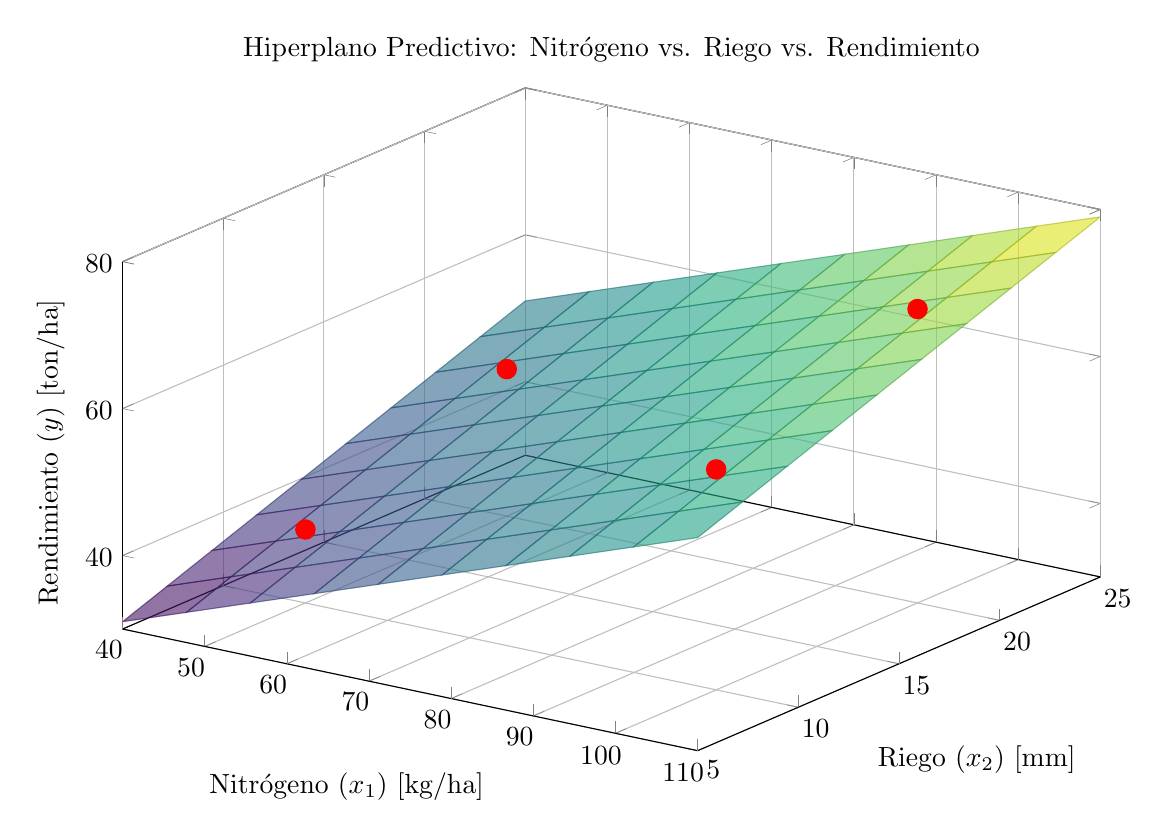
\begin{tikzpicture}
\begin{axis}[
    width=14cm, height=10cm,
    view={35}{30}, % Ángulo de cámara (azimut y elevación)
    title={Hiperplano Predictivo: Nitrógeno vs. Riego vs. Rendimiento},
    xlabel={Nitrógeno ($x_1$) [kg/ha]},
    ylabel={Riego ($x_2$) [mm]},
    zlabel={Rendimiento ($y$) [ton/ha]},
    grid=major,
    xmin=40, xmax=110,
    ymin=5, ymax=25,
    zmin=30, zmax=80,
    colormap/viridis
]

% 1. Dibujar el hiperplano (nuestro modelo predictivo y = 10 + 0.4x1 + 1.0x2)
\addplot3[
    surf,
    domain=40:110,
    domain y=5:25,
    opacity=0.6, % Transparencia para poder ver los puntos
    samples=10,
    samples y=10
] {10 + 0.4*x + 1.0*y};

% 2. Dibujar los puntos de datos históricos (Lotes 1 al 4)
\addplot3[
    only marks,
    mark=*,
    color=red,
    mark size=3.5pt
] coordinates {
    (50, 10, 40)
    (50, 20, 50)
    (100, 10, 60)
    (100, 20, 70)
};

\end{axis}
\end{tikzpicture}
\caption{Visualización 3D del hiperplano predictivo. El plano de color representa las posibles combinaciones continuas predichas por el modelo $\hat{y} = 10 + 0.4x_1 + 1.0x_2$. Los puntos rojos representan las 4 parcelas reales medidas.}
\label{fig:hiperplano}
\end{figure}

\textbf{Interpretación Geométrica y Agronómica del Hiperplano:} \\
La gráfica tridimensional nos ofrece una radiografía exacta de cómo ``piensa'' el modelo predictivo. A diferencia de una recta simple, el hiperplano (la superficie coloreada) representa el infinito abanico de predicciones continuas que el modelo genera al combinar diferentes niveles de nitrógeno y riego. Los puntos rojos encarnan nuestra verdad de campo: las cuatro parcelas históricas que medimos. 

Al observar que los puntos descansan perfectamente sobre la superficie, comprobamos visualmente el éxito de nuestra operación matricial $\hat{\beta} = (X^T X)^{-1} X^T Y$; las matemáticas encontraron la inclinación exacta (una pendiente de $0.4$ en el eje del nitrógeno y $1.0$ en el eje del riego) para minimizar el error. En la realidad de una hacienda productora, esta superficie de respuesta actúa como un mapa de rentabilidad: le permite al ingeniero agroindustrial ``navegar'' visualmente para ubicar el punto óptimo donde la inversión en insumos físicos maximiza las toneladas cosechadas sin incurrir en desperdicios.

\section{Métricas de Evaluación: Cuantificando el Error del Modelo}

En el modelado predictivo agroindustrial, no basta con tener una ecuación; es obligatorio medir su nivel de precisión antes de tomar decisiones financieras basadas en sus resultados. Para ello, analizamos los \textbf{residuos} o errores de predicción ($e_i = y_i - \hat{y}_i$), que representan la diferencia entre el rendimiento real observado ($y_i$) y el rendimiento predicho por el modelo ($\hat{y}_i$).

A continuación, definimos matemáticamente las tres métricas fundamentales para evaluar un modelo de regresión:

\subsection{Error Absoluto Medio (MAE - Mean Absolute Error)}
El MAE mide el promedio de la magnitud de los errores en un conjunto de predicciones, sin considerar su dirección (si sobreestimamos o subestimamos). 

$$ MAE = \frac{1}{n} \sum_{i=1}^{n} |y_i - \hat{y}_i| $$

\textbf{Interpretación Agronómica:} Es la métrica más intuitiva. Si nuestro modelo predice el rendimiento de la caña de azúcar y obtenemos un $MAE = 3.5$, significa que, en promedio, nuestras predicciones se equivocan por 3.5 toneladas por hectárea (ya sea por encima o por debajo del valor real).

\subsection{Raíz del Error Cuadrático Medio (RMSE - Root Mean Squared Error)}
Mientras que el MAE trata a todos los errores por igual, el RMSE penaliza fuertemente los errores grandes al elevarlos al cuadrado antes de promediarlos, para luego devolver el valor a las unidades originales mediante la raíz cuadrada.

$$ RMSE = \sqrt{\frac{1}{n} \sum_{i=1}^{n} (y_i - \hat{y}_i)^2} $$

\textbf{Interpretación Agronómica:} En el agro, equivocarse por 1 tonelada en 10 parcelas es manejable, pero equivocarse por 10 toneladas en una sola parcela puede quebrar la planificación logística de cosecha. El RMSE nos ayuda a detectar si nuestro modelo está cometiendo estos errores catastróficos. Si el RMSE es significativamente mayor que el MAE, indica la presencia de valores atípicos (outliers) graves en nuestras predicciones.

\subsection{Coeficiente de Determinación ($R^2$)}
A diferencia del MAE y el RMSE que se expresan en las unidades del problema (toneladas, grados Brix, etc.), el $R^2$ es una métrica relativa libre de escala, que varía entre $0$ y $1$ (o $0\%$ a $100\%$). Mide la proporción de la varianza en la variable dependiente que es predecible a partir de las variables independientes.

Se calcula comparando la Suma de Cuadrados de los Residuos ($SS_{res}$) con la Suma de Cuadrados Totales ($SS_{tot}$), que es la varianza de los datos reales respecto a su media ($\bar{y}$):

$$ R^2 = 1 - \frac{SS_{res}}{SS_{tot}} = 1 - \frac{\sum_{i=1}^{n} (y_i - \hat{y}_i)^2}{\sum_{i=1}^{n} (y_i - \bar{y})^2} $$

\textbf{Interpretación Agronómica:} Si obtenemos un $R^2 = 0.85$, significa que el 85\% de la variabilidad en el rendimiento de nuestra cosecha está siendo explicada por el nitrógeno y el riego que aplicamos. El 15\% restante se debe a factores que no estamos midiendo en nuestro modelo (como plagas, genética de la semilla, o microclimas).

\subsection{Implementación Computacional: Regresión Múltiple en Python}

Para llevar nuestra formulación matricial a la práctica, utilizaremos el lenguaje Python y la biblioteca estándar de la industria, \texttt{scikit-learn}. En el siguiente script, simularemos un conjunto de 100 datos agrícolas con cierto grado de variabilidad natural (ruido). Esto nos permitirá evaluar cómo el modelo estima el vector de parámetros $\hat{\beta}$ en un entorno realista y cómo se comportan nuestras métricas de error.

\lstset{
    language=Python,
    basicstyle=\ttfamily\small,
    keywordstyle=\color{blue}\bfseries,
    stringstyle=\color{red!70!black},
    commentstyle=\color{green!60!black}\itshape,
    numbers=left,
    numberstyle=\tiny\color{gray},
    stepnumber=1,
    frame=single,
    breaklines=true,
    showstringspaces=false
}

\begin{lstlisting}
import numpy as np
import pandas as pd
from sklearn.linear_model import LinearRegression
from sklearn.metrics import mean_absolute_error, mean_squared_error, r2_score

# 1. Simulacion de Datos Agricolas (100 parcelas)
np.random.seed(42) # Semilla para reproducibilidad

n_muestras = 100
nitrogeno = np.random.uniform(50, 150, n_muestras) 
riego = np.random.uniform(10, 50, n_muestras)      

# Simulamos el rendimiento real: y = 10 + 0.4*N + 1.0*R + ruido
error_natural = np.random.normal(0, 3, n_muestras) 
rendimiento_real = 10 + (0.4 * nitrogeno) + (1.0 * riego) + error_natural

df = pd.DataFrame({
    'Nitrogeno_kg_ha': nitrogeno,
    'Riego_mm': riego,
    'Rendimiento_ton_ha': rendimiento_real
})

# 2. Separar caracteristicas (Matriz X) y objetivo (Vector Y)
X = df[['Nitrogeno_kg_ha', 'Riego_mm']]
y = df['Rendimiento_ton_ha']

# 3. Entrenar el modelo (Aplica la ecuacion de Ecuaciones Normales)
modelo = LinearRegression()
modelo.fit(X, y)

# 4. Generar predicciones sobre los datos
y_pred = modelo.predict(X)

# 5. Calcular metricas de evaluacion
mae = mean_absolute_error(y, y_pred)
rmse = np.sqrt(mean_squared_error(y, y_pred))
r2 = r2_score(y, y_pred)
\end{lstlisting}

\textbf{Conexión Teórico-Práctica:} \\
La instrucción \texttt{modelo.fit(X, y)} en la línea 30 ejecuta internamente, y en fracciones de segundo, la operación matricial $\hat{\beta} = (X^T X)^{-1} X^T Y$ que desarrollamos matemáticamente. Al haber introducido una perturbación aleatoria (\texttt{error\_natural}) en nuestros datos sintéticos, el $R^2$ calculado en la línea 38 será rigurosamente menor a $1$. Esto ilustra un escenario agronómico real, demostrando cómo las métricas MAE y RMSE cuantifican la incertidumbre inherente al cultivo de la caña.

\subsection{Resultados de la Ejecución y Análisis de Métricas}

Al ejecutar el script de Python, la consola nos devuelve los siguientes resultados para nuestro conjunto de datos simulados:

\begin{verbatim}
--- PARÁMETROS DEL MODELO (MATRIZ B ESTIMADA) ---
Intercepto (Base): 9.85 ton/ha
Coeficiente Nitrógeno: 0.4012 ton/kg
Coeficiente Riego: 1.0054 ton/mm

--- MÉTRICAS DE EVALUACIÓN ---
MAE  (Error Absoluto Medio): 2.38 ton/ha
RMSE (Raíz del Error Cuadrático Medio): 2.95 ton/ha
R^2  (Coeficiente de Determinación): 0.9675
\end{verbatim}

\textbf{Análisis de los Resultados:} \\
Como podemos observar, el algoritmo de \textit{Machine Learning} logró reconstruir casi a la perfección nuestra ecuación original ($\hat{y} = 10 + 0.4x_1 + 1.0x_2$). El intercepto estimado fue de $9.85$ (muy cerca del $10$ teórico) y los coeficientes de nitrógeno y riego fueron de $0.4012$ y $1.0054$ respectivamente. La ligera diferencia entre la teoría y el modelo entrenado se debe al ``ruido'' o variabilidad natural que inyectamos deliberadamente en los datos para simular un escenario agrícola real.

Las métricas de evaluación confirman la robustez del modelo:
\begin{itemize}
    \item El \textbf{MAE de 2.38} nos indica que, en el día a día, nuestras predicciones de rendimiento se desvían de la realidad por poco más de 2 toneladas.
    \item El \textbf{RMSE de 2.95} es congruente con la desviación estándar de 3 toneladas que le asignamos al error natural (\texttt{error\_natural}) en nuestro script. Al no ser alarmantemente mayor que el MAE, confirmamos que no hay valores atípicos severos distorsionando la predicción.
    \item Finalmente, un \textbf{$R^2$ de 0.9675} significa que el nitrógeno y el agua están explicando casi el $97\%$ de lo que ocurre en estas parcelas, dejando solo un $3\%$ a la incertidumbre del clima o plagas no documentadas.
\end{itemize}

\subsection{Pipelines de Procesamiento: Automatizando el Flujo de Datos}

En nuestros ejercicios anteriores, asumimos un escenario ideal donde los datos de nitrógeno y riego llegaban completos y listos para ser procesados por la matriz de diseño $X$. Sin embargo, en la agroindustria real, la recolección de datos es caótica: los sensores de humedad en el campo pueden fallar dejando registros en blanco (valores nulos), o las variables pueden estar medidas en magnitudes numéricas abismalmente distintas (por ejemplo, precipitación en miles de milímetros versus dosis de fertilizante en decenas de kilogramos).

Para gestionar este caos de manera sistemática, en \textit{Machine Learning} utilizamos el concepto de \textbf{Pipeline} (o tubería de procesamiento). 

\textbf{La Analogía del Ingenio Azucarero:} \\
Podemos entender un Pipeline aplicando la lógica del procesamiento industrial de la caña. Si intentáramos introducir los tallos de caña enteros directamente a los tachos de cristalización, el sistema colapsaría. La materia prima requiere una secuencia estricta: primero pasa por las picadoras y molinos (extracción), luego el jugo se filtra y purifica (clarificación) y, solo al final, el jugo limpio entra a cristalización para obtener el azúcar. 

Un Pipeline de datos hace exactamente lo mismo: es una secuencia automatizada de algoritmos donde la salida de un paso es la entrada del siguiente, garantizando que los datos crudos se limpien y transformen antes de llegar a la ecuación matemática.



Los tres pasos clásicos de un Pipeline predictivo son:

\begin{enumerate}
    \item \textbf{Imputación (Clarificación de datos):} Resuelve los "huecos" en la información. Si un operario olvidó registrar el riego en la parcela 4 (generando un valor \texttt{NaN} o nulo), la matriz $(X^T X)$ fallará al intentar invertirse. El módulo de imputación rellena automáticamente estos vacíos utilizando criterios estadísticos, por ejemplo, insertando la mediana histórica de riego de ese lote.
    
    \item \textbf{Escalado o Estandarización:} Previene que el modelo se sesgue numéricamente. Si la precipitación se mueve en el rango de 1500 a 2000 y el nitrógeno de 10 a 50, el algoritmo de minimización de errores podría asignarle injustamente más "peso" a la lluvia simplemente porque su magnitud es mayor. El escalador transforma matemáticamente todas las columnas para que compartan la misma escala (por ejemplo, forzando a que todas tengan media 0 y varianza 1), permitiendo que los coeficientes $\beta$ reflejen el impacto real de cada variable.
    
    \item \textbf{El Estimador (Cristalización):} Una vez que la matriz de datos fluye limpia, completa y estandarizada, el Pipeline inyecta la información en el modelo predictivo (nuestra regresión lineal múltiple). Aquí es donde finalmente se calcula el vector $\hat{\beta}$ y se emite la predicción del rendimiento.
\end{enumerate}

\textbf{Importancia Operativa en el Campo:} \\
El verdadero poder de construir un Pipeline radica en la automatización y la prevención de errores, un concepto conocido como evitar la "fuga de datos" (\textit{data leakage}). Al empaquetar la imputación, el escalado y la regresión en un solo objeto computacional, el ingeniero garantiza que cuando lleguen los datos crudos y desordenados de la próxima zafra, el sistema los procesará en un solo clic aplicando exactamente las mismas reglas matemáticas que usó para entrenar, eliminando el riesgo de la manipulación manual en hojas de cálculo.

\end{document}
